\section{Transfer and published comparison}
\label{sec:transfer}
We now freeze every choice on VOC-Sim and score COCO-Cap. The confirmed all-call training-free pipeline gives 0.637 mIoU; the later joint temporal selection gives 0.644. COCO-Cap includes captions in which the queried class name is absent, so separate class-word attribution is important. Neither the temporal window nor the threshold is chosen on COCO-Cap.

\begin{figure*}[t]
\centering
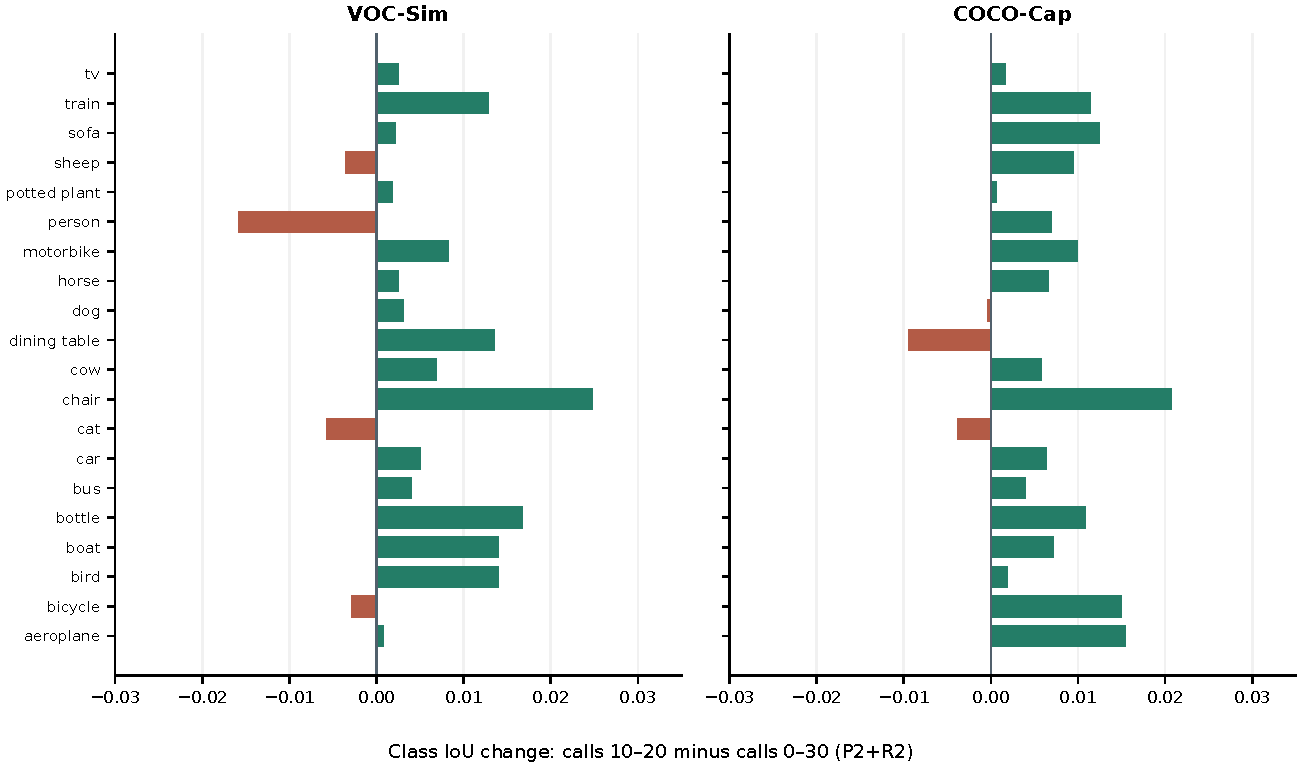
\includegraphics[width=.87\textwidth]{figures/temporal_class_effects.pdf}
\caption{\textbf{The middle-call gain is heterogeneous.} Per-class IoU change for MID-P2+R2 versus ALL-P2+R2 in the same SG22 evaluation, with the threshold chosen on VOC only. Chair improves on both datasets; VOC person loses 0.016. Positive overall mIoU does not imply every class improves.}
\label{fig:temporal_classes}
\end{figure*}

\begin{table}[t]
\centering
\footnotesize\setlength{\tabcolsep}{3pt}
\begin{tabular}{@{}lcc@{}}
\toprule
Method & VOC-Sim & COCO-Cap \\
\midrule
\multicolumn{3}{@{}l}{\emph{Published in OVAM, Table 1}}\\
DAAM & .662 & .484 \\
Attn2Mask & .687 & .550 \\
OVAM, class word & .704 & .582 \\
\midrule
\multicolumn{3}{@{}l}{\emph{Published methods with extra training}}\\
Grounded Diffusion & .621 & .502 \\
DatasetDM & .803 & .593 \\
\midrule
\multicolumn{3}{@{}l}{\emph{Ours, regenerated images / released annotations}}\\
All-call P2+R2 & .813$^{\dagger}$ & .637$^{*}$ \\
Middle-call P2+R2 & .817$^{\dagger}$ & .644$^{*}$ \\
A3 middle-call P2+R2$^{\ddagger}$ & .823$^{\dagger}$ & .662$^{*}$ \\
\bottomrule
\end{tabular}
\caption{\textbf{Class-word results against the numbers reported by OVAM}~\cite{marcosmanchon2024ovam}; optimized-token rows are deliberately excluded. OVAM Table 1 evaluates each baseline on its authors' renders and annotations, whereas our attention requires regeneration from prompts and seeds and uses the released annotations. Thus cross-block differences are indicative, not a paired head-to-head estimate. $^{\dagger}$VOC OOF; $^*$COCO with VOC-frozen threshold and method. $^{\ddagger}$Exploratory forced-OOF A3 result; it was not the registered multi-candidate winner and uses the implemented transposed-affinity score.}
\label{tab:published_comparison}
\end{table}

The published OVAM table is the appropriate literature context, but its rows cannot be interpreted as a controlled paired test of our operator: different generation settings can alter the image, and OVAM's evaluation adapts prompt-bound methods to an attribution prompt on COCO-Cap. We additionally re-scored released masks with available evaluation code; those scores and their method-specific conditions remain in the artifact registry rather than replacing the paper's published numbers.

\paragraph{What later extensions show.}
After the validated MID-P2+R2 choice, the SG24 A3 weighted CA seed reaches 0.823 forced OOF versus 0.817 for its same-run unweighted reference and 0.662 versus 0.644 on COCO-Cap. Its full-VOC threshold gives 0.824, which is an in-sample score and is not used as the main VOC estimate. A subsequent multiscale SA experiment keeps A3 fixed: 16-to-64-pixel propagation plus R2 gives 0.818 VOC OOF and 0.697 frozen COCO, while the 64-pixel reference gives 0.823 and 0.662. It is a transfer observation, not the VOC-selected method. A broad SG27 fusion screen also retains the fine-scale reference in all five folds; its largest COCO score is not promoted because it loses VOC and has a boundary threshold. These studies expose a meaningful scale-versus-transfer tradeoff without changing the confirmed paper result.
